\section{\name Framework}\label{sec:framework}

% \method optimizes AD kernels by jointly refining forward computation, backward computation, and their saved-state interface. Users supply the target kernels, a model, and prepared workload configurations. The model and workloads support model-level verification and evaluation; the output is selected forward--backward kernel implementations with their deployment bindings. The seed synthesizer exposes the joint implementation space; the evolver explores it; and the verifier and evaluator determine numerical acceptance and training benefit.

\system integrates agentic kernel development with PyTorch's compiler and runtime. It takes target computations from a training workload, constructs executable forward--backward implementations for agentic optimization, and deploys the optimized implementations back into the training framework for verification and evaluation.

% \subsection{Contract and Design Overview}
\subsection{System Overview}
\label{sec:design_overview}

\noindent\textbf{Input and Output.}
% Given a PyTorch model, a training workload, and a set of target operators to optimize, \system returns optimized forward--backward implementations and their deployment bindings. Formally, the system input is $\mathcal I=(\mathcal O,M,W)$, where $\mathcal O$ specifies the target computations, which can be primitive operators (e.g., normalization and activation) or composite operators (e.g., an MLP block), $M$ denotes the model, and $W$ specifies the training workload, including training data, loss computation, batch and input settings, precision, optimizer settings, and target device. The target operators and their integration sites in the model are specified in advance. 
The system input is $\mathcal I=(\mathcal O,M,W)$, where $\mathcal O$ specifies the target computations, which can be primitive operators (e.g., normalization and activation) or composite operators (e.g., an MLP block), $M$ denotes the model, and $W$ specifies the training workload, including training data, loss computation, batch and input settings, precision, optimizer settings, execution settings, and target device. The target operators and their integration sites in the model are specified in advance.

% \noindent\textbf{Training-implementation contract.}
% \label{sec:kernel-task}
% The specified primitive or composite operators define the kernel-optimization targets. Each kernel task is defined by its reference computation and configuration. The supplied model and prepared workload provide the context for verifying candidates and measuring their training impact; tasks with the same computation and configuration may be assessed in different training contexts. Section~\ref{sec:target_preparation} describes the prepared workloads and target operators.
Each kernel optimization task is defined by its reference computation $f$ and configuration $c$. The model and training workload provide the context for verifying and evaluating optimized implementations. Thus, the same kernel task may be assessed in different training contexts. Section~\ref{sec:target_preparation} describes how kernel tasks and their associated workloads are constructed.

The returned set of implementations is
\begin{equation}
    \mathcal K_{\mathrm{selected}}
    =\{(p_i,c_i,\sigma_i)\mid i\in I_{\mathrm{selected}}\},
    \label{eq:selected_kernels}
\end{equation}
where $p_i$ contains a forward--backward implementation and its saved-state contract, $c_i$ is its supported configuration, and $\sigma_i$ binds it to the declared model sites. 
% The verifier and evaluator select these implementations using their deployment evidence. 
Candidates are installed in the supplied model for verification and evaluation; the system returns optimized kernels and their deployment bindings. 
Targets without qualifying replacements retain their reference implementations, and an empty selected set indicates that no optimized kernel deployment qualified.
% For each target operator, \system seeks an optimized forward--backward implementation that satisfies the correctness requirements and provides performance benefits in the target training workload. The system returns the selected implementations, their supported configurations, and deployment bindings that specify where they replace the original computations in the model. Operators without qualifying replacements retain their original implementations. 
For example, given a SwiGLU MLP as the target operator, Qwen3-0.6B as the model, and a WikiText-2 training workload, \system constructs an editable MLP implementation, jointly optimizes its forward and backward computations, and verifies and evaluates the resulting implementation within Qwen3-0.6B before accepting it for deployment.

\noindent
\textbf{Workflow.}
Figure~\ref{fig:evograd_pipeline} summarizes the architecture of \system. The synthesis and evolution stages construct a candidate as follows:
\begin{equation}
    \begin{aligned}
    (f,c)
    &\xrightarrow{\mathrm{AOTAutograd}}
    G_{f,c}
    \xrightarrow{\mathrm{compiler\ guided\ partition}}
    (L,R)\\
    &\xrightarrow{\mathrm{semantic\ synthesis}}
    p_0
    \xrightarrow{\mathrm{evolution}}
    p^\star,
    \end{aligned}
    \label{eq:evograd_pipeline}
\end{equation}
where $G_{f,c}$ is the joint forward--backward ATen graph and $p_0$ is the synthesized seed.

\begin{figure}
    \centering
    % 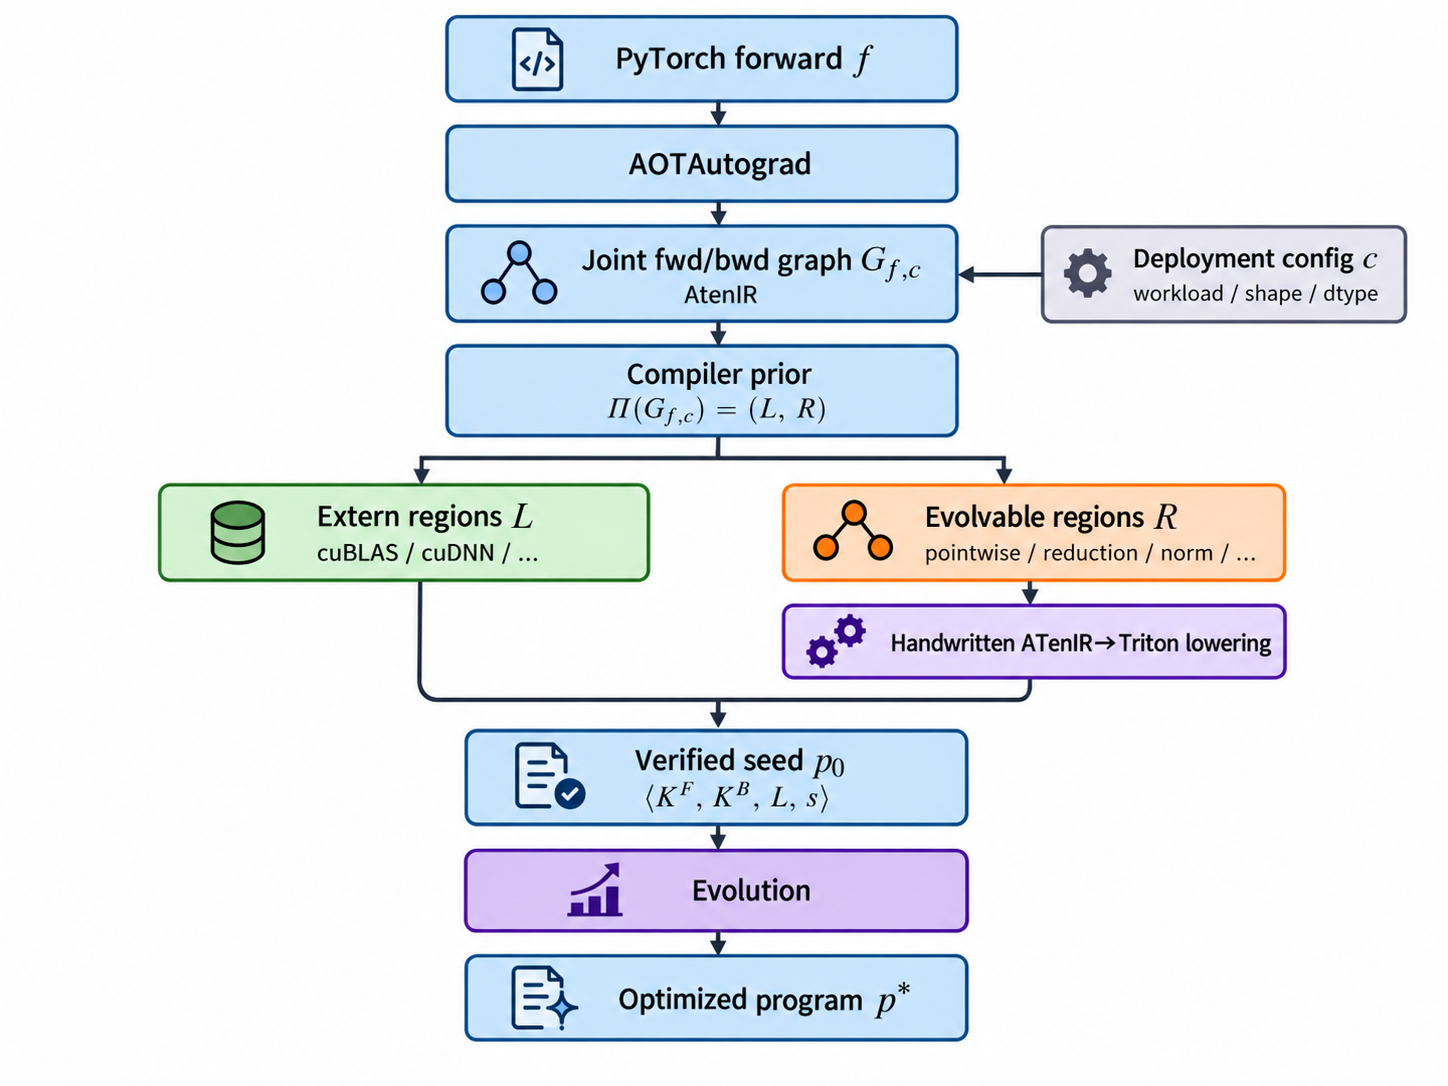
\includegraphics[width=\linewidth]{figures/evograd_pipeline.png}
    % Framework overview. The original seed-synthesis figure is retained alongside
% this editable diagram; the third stage makes deployment assessment explicit.
\begingroup
\small
\setlength{\fboxsep}{5pt}
\begin{tabular}{@{}c@{}}
PyTorch forward $f$ + workload configuration $c$ \\
$\downarrow$ \\
\fbox{\parbox{0.91\linewidth}{\centering
    \textbf{1. Seed synthesizer}\\[2pt]
    AOTAutograd $\rightarrow$ AtenIR $\rightarrow$ partition $(L,R)$\\
    Preserve library calls $L$; lower $R$ to Triton primitives
}} \\
$\downarrow\; p_0=\langle K_0^F,K_0^B,L,s_0\rangle$ \\
\fbox{\parbox{0.91\linewidth}{\centering
    \textbf{2. Agentic evolver}\\[2pt]
    Jointly refine forward, backward, and saved state\\
    $\circlearrowleft$ Local correctness checks and latency--memory score
}} \\
$\downarrow$ \\
\fbox{\parbox{0.91\linewidth}{\centering
    \textbf{3. Verifier + evaluator}\\[2pt]
    Check pair, integration, and training behavior\\
    Measure operator and training latency and memory\\
    Select qualifying replacements; reverify their combination
}} \\
$\downarrow$ \\
Accepted deployments with training measurements
\end{tabular}
\endgroup

    \caption{\method optimizes target AD kernels through compiler-guided synthesis and evolution, returning selected kernel implementations and bindings. The supplied model and workload support model-level verification and evaluation. Local checks and scores guide search; training measurements select qualifying replacements, whose combined deployment is verified again. External-library regions $L$ remain preserved.}
    \minjia{Please redraw the system overview figure to reflect our new framing. Instead dof showing ADopt as a standalone pipeline of seed synthesis, evolution, and verification/evaluation, we should explicitly show how ADopt integrates with PyTorch's compiler and runtime. The figure should show how ADopt starts from target operators in a PyTorch training workload, uses compiler-derived semantics to construct editable AD seeds, jointly optimizes forward/backward implementations and saved state, and integrates the generated kernels back into PyTorch for verification, evaluation, and deployment. Please also distinguish the lightweight feedback loop during agentic search from the more comprehensive deployment-time assessment, and make it clear where ADopt-Bench fits into this workflow. The key message is that ADopt develops kernels within the training framework in which they will be deployed.}
    \label{fig:evograd_pipeline}
\end{figure}

% \noindent\textbf{Training-implementation contract.}
% \label{sec:kernel-task}
% The specified primitive or composite operators define the kernel-optimization targets. Each kernel task is defined by its reference computation and configuration. The supplied model and prepared workload provide the context for verifying candidates and measuring their training impact; tasks with the same computation and configuration may be assessed in different training contexts. Section~\ref{sec:target_preparation} describes the prepared workloads and target operators.

% \noindent\textbf{Candidate implementation.}
% Each kernel task produces a candidate implementation $p$ comprising GPU kernels and forward and backward host code, $F_p$ and $B_p$, that launch them. \Appref{app:task_format} illustrates the task and deployment interfaces. Under configuration $c$, they satisfy
% \begin{equation}
%     (y,s_p)=F_p(x,\theta), \qquad
%     (\nabla_x,\nabla_\theta)=B_p(\nabla_y,s_p).
%     \label{eq:autograd_contract}
% \end{equation}
% Here, $s_p$ contains the state retained by $F_p$ for use in $B_p$, with its tensors determining the explicitly saved memory. The backward implementation returns the required vector--Jacobian products $\nabla_x=(\partial f/\partial x)^{\top}\nabla_y$ and $\nabla_\theta=(\partial f/\partial\theta)^{\top}\nabla_y$. Candidates may optimize forward and backward algorithms, fusion boundaries, which intermediates to retain or recompute, and permitted vendor-library calls. The pair is deployed through a \texttt{torch.autograd.Function}, allowing PyTorch autograd to invoke $B_p$ when the candidate runs as an operator or within its source model.

% \noindent\textbf{Selected output.}
% The returned set of implementations is
% \begin{equation}
%     \mathcal K_{\mathrm{selected}}
%     =\{(p_i,c_i,\sigma_i)\mid i\in I_{\mathrm{selected}}\},
%     \label{eq:selected_kernels}
% \end{equation}
% where $p_i$ contains a forward--backward implementation and its saved-state contract, $c_i$ is its supported configuration, and $\sigma_i$ binds it to the declared model sites. The verifier and evaluator select these implementations using their deployment evidence. Candidates are installed in the supplied model for verification and evaluation; the system returns optimized kernels and their deployment bindings. Targets without qualifying replacements retain their reference implementations, and an empty selected set indicates that no optimized kernel deployment qualified.

% For example, given a SwiGLU MLP kernel target, Qwen3-0.6B, and a prepared WikiText-2 workload, \method synthesizes and evolves the MLP implementation, verifies and evaluates it at the declared model sites, and returns a qualifying kernel implementation with its bindings.

% For a task $(f,c)$, \method searches the permitted program space $\mathcal{P}_{f,c}$. Reimplementing computations already served by mature vendor libraries adds unnecessary search effort, but directly evolving compiler-generated Triton code inherits the compiler's kernel boundaries, lowering, and scheduling decisions. \method instead preserves compiler-selected library calls while reconstructing the remaining computation from ATen semantics.





% \subsection{Compiler-Guided Seed Synthesizer}
\subsection{Compiler-Guided Seed Synthesis}
\label{sec:seed_synthesis}

% For each selected operator/configuration, the seed synthesizer constructs a structured starting program from training semantics, exposing joint forward--backward implementation choices without discarding compiler-selected library code.

The goal of seed synthesis is to construct a starting program that captures the semantics of a training operator while facilitating agentic optimization of its implementation. A natural approach is to provide the agent with the original PyTorch implementation and let it generate optimized forward and backward kernels. However, the backward computation and its dependencies on forward intermediates are implicit in the original implementation. The agent must derive these computations, determine their numerical requirements, and construct the saved-state interface before optimizing the kernels.

Another approach is to start from the GPU kernels generated by PyTorch's compiler. These kernels provide optimized implementations of the forward and backward computations. However, they represent one particular realization of the underlying AD computation, including specific kernel boundaries, computation strategies, and saved-state choices. For agentic optimization, we seek a program representation that preserves the underlying AD semantics while exposing these implementation choices as part of the search space.

\name constructs such a representation by leveraging the program semantics available in PyTorch's compiler. It synthesizes an executable forward--backward program, retains selected optimized library implementations, and exposes the remaining computations and saved-state interface to agentic optimization.

\noindent
\textbf{Forward--backward program representation.}
For each selected operator configuration, the kernel task provides a reference PyTorch forward computation, $y=f(x,\theta)$, where $x=(x_1,\ldots,x_n)$ is a tuple of input tensors, $\theta=(\theta_1,\ldots,\theta_m)$ a tuple of trainable parameter tensors, and $y=(y_1,\ldots,y_k)$ a tuple of forward outputs. The specification identifies the required outputs and the differentiable inputs and parameters for which gradients must be produced. Reference gradients are computed through PyTorch autograd with supplied upstream gradients $\nabla_y=(\nabla_{y_1},\ldots,\nabla_{y_k})$, one for each output. Each task fixes a configuration $c$ specifying tensor shapes, dtypes, memory layouts, and static operator parameters such as normalization epsilon. It is derived from the source-model training workload (Section~\ref{sec:workload_configs}). Static parameters remain fixed in $f$, while $x$, $\theta$, and $\nabla_y$ vary across instances. Reproducible generators support search-time timing, while recorded $(x,\theta,\nabla_y)$ instances from source-model execution supply verification and formal operator timing inputs in their original memory layouts.

\noindent\textbf{Candidate implementation.}
Each kernel task produces a candidate implementation $p$ comprising GPU kernels and forward and backward host code, $F_p$ and $B_p$, that launch them. \Appref{app:task_format} illustrates the task and deployment interfaces. Under configuration $c$, they satisfy
\begin{equation}
    (y,s_p)=F_p(x,\theta), \qquad
    (\nabla_x,\nabla_\theta)=B_p(\nabla_y,s_p).
    \label{eq:autograd_contract}
\end{equation}
Here, $s_p$ contains the state retained by $F_p$ for use in $B_p$, with its tensors determining the explicitly saved memory. The backward implementation returns the required vector--Jacobian products $\nabla_x=(\partial f/\partial x)^{\top}\nabla_y$ and $\nabla_\theta=(\partial f/\partial\theta)^{\top}\nabla_y$. Candidates may optimize forward and backward algorithms, fusion boundaries, which intermediates to retain or recompute, and permitted vendor-library calls. The pair is deployed through a \texttt{torch.autograd.Function}, allowing PyTorch autograd to invoke $B_p$ when the candidate runs as an operator or within its source model.

% \noindent\textbf{Autograd semantic extraction.}
\noindent\textbf{Extracting AD semantics.}
AOTAutograd derives the forward and backward computation of $f$ under configuration $c$. We represent it in AtenIR, a graph capturing ATen operators (e.g., \texttt{aten.add}, \texttt{aten.sum}, and \texttt{aten.mm}) and their data dependencies, without committing to kernel boundaries or schedules. Applying PyTorch's \texttt{min\_cut\_rematerialization\_partition} to the joint graph initializes the saved-state interface.

\noindent\textbf{Compiler-aware partitioning.}
For a task $(f,c)$, \method searches the permitted program space $\mathcal{P}_{f,c}$. Reimplementing computations already served by mature vendor libraries adds unnecessary search effort, but directly evolving compiler-generated Triton code inherits the compiler's kernel boundaries, lowering, and scheduling decisions. \method instead preserves compiler-selected library calls while reconstructing the remaining computation from ATen semantics.
We inspect TorchInductor's lowering decisions to partition the forward--backward computation as
\begin{equation}
    \Pi(G_{f,c}) = (L,R),
    \label{eq:partition}
\end{equation}
retaining its external-library assignments for operations such as dense GEMMs and convolutions backed by cuBLAS and cuDNN.

\noindent\textbf{Semantic resynthesis.}
For $R$, handwritten lowering rules map supported AtenIR operations to pre-implemented Triton primitives and generate host code that invokes them according to data dependencies. The primitives and host code implement broadcasting, dtype conversion, and reduction semantics. This deterministically constructs the seed without LLM-based synthesis or cross-operator fusion; its primitive boundaries remain open to rewriting during evolution. Combining the synthesized computation with $L$ yields
\begin{equation}
    p_0 =
    \left\langle
        K_0^F,\,
        K_0^B,\,
        L,\,
        s_0
    \right\rangle,
    \label{eq:seed_program}
\end{equation}
where $K_0^F$ and $K_0^B$ denote the synthesized forward and backward kernels with their host code, $L$ contains the preserved library calls, and $s_0$ is the state passed from forward to backward. \Appref{app:seed_example} illustrates these components with a masked linear map.

\noindent\textbf{Constructing the search space.} 
% Let $L$ denote the preserved external-library regions, $R$ the remaining ATen computation, and $\mathcal{P}_{f,c}^{L}\subseteq\mathcal{P}_{f,c}$ the candidate space that preserves $L$ while allowing different implementations and saved-state choices for $R$. 
Let $L$ denote the computations served by the preserved external library calls and $R$ denote the remaining ATen computations. For a target computation $f$ and configuration $c$, the synthesized seed defines an implementation space $\mathcal{P}_{f,c}^{L}$ in which the agent can explore alternative kernel implementations, fusion strategies, and saved-state representations for $R$ while retaining the optimized library calls in $L$ and preserving the external AD contract.


\subsection{Agentic Evolver}
\label{sec:evolution}

An AD kernel replaces both the forward and backward implementations of a differentiable operator in the training framework. Its optimization objective must therefore account for the combined execution latency of both passes and the memory required to retain intermediate state between them. Given a compiler-guided seed, \method jointly optimizes the forward and backward implementations and their saved-state interface while preserving the operator's external AD semantics.

Given the synthesized seed and its associated implementation space $\mathcal{P}_{f,c}^{L}$, \method searches for an implementation that improves forward-backward execution efficiency while reducing saved-state memory. The objective is
\begin{equation}
    p^\star
    \in
    \operatorname*{arg\,max}_{p\in\mathcal{P}_{f,c}^{L}}
    \operatorname{Score}(p;c)
    \quad \text{subject to} \quad
    \mathcal{V}(p,f,c)=1,
    \label{eq:objective}
\end{equation}
where $\operatorname{Score}(p;c)=Q(p;c)$ is the Tier~1 search score in Equation~\ref{eq:tier1_search_score}, and $\mathcal{V}$ is the verification predicate in Equation~\ref{eq:validity}. This objective guides local search; the evaluator subsequently uses training measurements to select qualifying replacements for combined deployment.

% The synthesized pair provides a checked starting implementation; evolution explores alternative kernels, orchestration, and saved-state representations. 
Unlike conventional kernel optimization workflows that operate on individual GPU kernels, \method presents the complete forward--backward program to the agent as the unit of optimization. The program includes the GPU kernels, host code that orchestrates their execution, external library calls, and the state passed between the forward and backward computations.
Starting from the verified seed $p_0$, \method uses OpenEvolve to optimize Equation~\ref{eq:objective}. Search can modify the synthesized Triton kernels, host code, and saved-state policy while preserving $L$ and the public autograd interface. Candidates must pass search-time correctness checks before timing and scoring; failures are rejected. Selected final candidates undergo the applicable verification and evaluation protocols in Sections~\ref{sec:verification_protocol} and~\ref{sec:evaluation_protocol}.

\minjia{I think this is one of the most important parts of the paper, but currently I don't get a good sense of how the agent actually optimizes an AD kernel. What does the agent see? What can it change? What feedback does it receive, and how does that feedback help it improve the implementation? It would be also interesting to walk through a real example where the agent makes coordinated changes to the forward and backward computations or redesigns the saved state. This would help readers understand what joint optimization actually buys us. Finally, clarify which parts of the workflow are specific to ADopt and which are provided by the underlying evolver. Ideally, OpenEvolve is just one instance of the agentic optimization framework, not an essential part of our design.}

% \subsection{Deployment Verifier}
\subsection{Progressive Correctness Verification}
\label{sec:verification_protocol}

Verifying an agent-generated AD kernel requires more than checking its forward and backward pass in isolation. The implementation must also behave correctly when invoked by PyTorch's autograd engine, interact with other operators in the model, preserve numerical accuracy across training updates. However, verifying every candidate through whole model training would be expensive. \system there uses progressive verification, with three levels of increasing execution scope and verification cost:
% \method uses three verification gates: 
% local pair verification, single-step framework integration verification, 
local AD kernel verification, framework integration verification, and multi-step training verification,
\minjia{I added the rationale for this progressive verification protocol and also updated the names of the three verification steps. Please update the following notations, perhaps local, int, train, and make sure the notations are consistent.}
% and multi-step training verification, 
with binary outcomes $\mathcal{V}_{\mathrm{pair}}$, $\mathcal{V}_{\mathrm{int}}$, and $\mathcal{V}_{\mathrm{train}}$, respectively.
The applicable gate set $\mathcal{G}_{f,c}$ depends on the target granularity and the supplied model/workload. For candidates satisfying the task's static rules, acceptance requires
\begin{equation}
    \mathcal{V}(p,f,c)
    =
    \bigwedge_{g\in\mathcal{G}_{f,c}}
    \mathcal{V}_g(p,f,c)
    =1.
    \label{eq:validity}
\end{equation}
Pair verification asks whether the forward--backward pair computes the declared function. Integration verification asks whether the candidate remains accurate when deployed through PyTorch autograd, as an operator and within the source model. Training verification asks whether its numerical differences compound over successive optimizer updates. A gate passes only if the candidate executes completely and meets every structural and numerical criterion.

Floating-point arithmetic admits no single correct result: two correct implementations of the same computation differ by rounding, and a model can amplify such differences. Every numerical criterion therefore takes the same form: the candidate's error must not exceed the larger of a fixed floor and a multiple of the error of trusted implementations of the same computation, measured on the same inputs. The trusted implementations are the source model's native execution and its \texttt{torch.compile} compilation; thresholds depend only on them, never on the candidate. 

During search, the evolver applies Gate~1 to a subset of the recorded calls to admit candidates for scoring; deployment verification then runs the full gates. A primitive candidate must pass pair verification and operator-scope integration verification. A composite candidate must additionally pass model-scope integration and training verification where available, with the candidate installed alone at its site in the supplied model. Selected composite candidates deployed together are verified again by model-scope integration and training verification. Only deployments passing all required gates contribute to the main performance results. All verification uses PyTorch's deterministic settings and runs outside timed regions. Model-specific gate availability, configurations, and detailed procedures are provided in \appref{app:verification_details}.

\noindent\textbf{Gate 1: Local pair verification ($\mathcal{V}_{\mathrm{pair}}$).}
Gate~1 asks whether the pair computes the declared function. It directly invokes the candidate's forward and backward implementations, $F_p$ and $B_p$, with $B_p$ consuming the candidate's own saved state $s_p$, and compares every declared forward output and the gradient of every differentiable input and parameter with the reference computation $f$ under PyTorch autograd; the internal decomposition and saved state need not match the reference.

The gate replays calls recorded from source-model training on real-world datasets, preserving their inputs, parameters, upstream gradients, and memory layouts. For each such tensor $z$, the reference $z^{\mathrm{ref}}$ is $f$ evaluated in float32, so that a candidate is not penalized for being more accurate than the model's reduced-precision arithmetic, and $z^{\mathrm{native}}$ is $f$ at the model's own dtypes. With $d(a,b)=\|a-b\|_\infty/\|b\|_\infty$, the candidate must satisfy on every call
\begin{equation}
d(z^{\mathrm{cand}},z^{\mathrm{ref}})
\leq \max\Bigl\{\beta_1,\;\gamma_1\max_{\mathrm{calls}}d(z^{\mathrm{native}},z^{\mathrm{ref}})\Bigr\},
\label{eq:local_numerical_contract}
\end{equation}
where $\beta_1$ is a floor fixed per dtype and $\gamma_1=2$ is a safety margin, as in the kernel tests of FlashAttention~\cite{dao2022flashattention}. The floor decides for most results; the native term takes over where large terms nearly cancel, as in attention gradients, and native execution itself exceeds the floor. Acceptance also requires the declared structure, shape, and dtype, finite results, and no input mutation unless permitted by the task.


\noindent\textbf{Gate 2: Framework integration verification ($\mathcal{V}_{\mathrm{int}}$).}
Gate~2 checks the candidate through its deployment path in PyTorch autograd. At \emph{operator scope}, it replays recorded calls and compares the same outputs and gradients as Gate~1, isolating local error. At \emph{model scope}, it compares model outputs, loss, and every trainable parameter's gradient, capturing error propagation and interactions among replacements. Each replaced site then receives inputs computed by the modified model, allowing local errors to affect downstream computations and exposing deployment faults such as skipped sites. Candidate and native eager executions perform one forward and backward pass under matched inputs, parameters, random states, and numerical settings, without an optimizer update.

A sample $x$ is one recorded call at operator scope and one workload batch at model scope. For each required floating-point result tensor $z$, we measure
\begin{equation}
\begin{aligned}
E_2(z;x)
&=\frac{\|z_x^{\mathrm{cand}}-z_x^{\mathrm{ref}}\|_2}{\max(\|z_x^{\mathrm{ref}}\|_2,\epsilon)},\\
E_{\max}(z;x)
&=\frac{\|z_x^{\mathrm{cand}}-z_x^{\mathrm{ref}}\|_\infty}{\max(\operatorname{RMS}(z_x^{\mathrm{ref}}),\epsilon)},
\end{aligned}
\label{eq:integration_errors}
\end{equation}
where $\operatorname{RMS}(z)=\sqrt{n_z^{-1}\sum_i z_i^2}$ over the $n_z$ elements of $z$, and $\epsilon=10^{-30}$ guards against division by zero. $E_2$ measures error across the tensor, including small discrepancies spread across many elements; $E_{\max}$ catches errors confined to a few elements that contribute little to $E_2$. Its normalization uses the tensor's typical magnitude rather than individual near-zero elements.

For each result tensor $z$ and metric $m\in\{2,\max\}$, let $D_m(z;x)$ be the larger of the native-repeat and compile--native discrepancies on calibration sample $x$. The threshold is
\begin{equation}
T_{z,m}=\gamma\max\left\{\max_{x\in\mathcal{C}}D_m(z;x),\,f_{z,m}\right\},
\label{eq:integration_calibration}
\end{equation}
where $\mathcal{C}$ is the calibration set, $f_{z,m}>0$ is a floor, and $\gamma>1$ is a fixed scope-specific safety margin. Operator scope uses separate calibration and acceptance calls; model scope verifies fresh executions of the calibrated inputs. Every required result on every verification sample must satisfy
\begin{equation}
E_2(z;x)\leq T_{z,2}
\quad\land\quad
E_{\max}(z;x)\leq T_{z,\max},
\label{eq:integration_acceptance}
\end{equation}
together with Gate~1's structure, shape, dtype, finiteness, and input-mutation checks. Model scope additionally requires unchanged parameters and the declared call count at every replaced site.

\noindent\textbf{Gate 3: Multi-step training verification ($\mathcal{V}_{\mathrm{train}}$).}
Gate~3 checks whether numerical differences compound through successive gradient computations and optimizer updates on real-world datasets. Each update changes the weights and optimizer state used by later steps, allowing differences that are small in a single forward--backward pass to grow along the training trajectory. Where available, it follows Gates~1 and~2 for individual composite candidates and their combined deployments. Candidate and native eager runs start from identical model and optimizer states and use the same training batches, random states, numerical settings, and optimizer schedule. Neither run is reset to the other's state.

Let $\ell_t^p$ be the training loss differentiated at update $t$ of run $p$, and let $d_t^p=\ell_t^p-\ell_t^{\mathrm{native}}$. Over all $N$ updates, we measure
\begin{equation}
R_p=\sqrt{\frac{1}{N}\sum_{t=1}^{N}(d_t^p)^2},
\qquad
M_p=\max_{1\leq t\leq N}|d_t^p|.
\label{eq:training_errors}
\end{equation}
$R_p$ measures the root mean square loss difference, preventing cancellation across updates; $M_p$ bounds the largest single-step difference. Both use the full trajectory, without windows or excluded steps.

Acceptance requires
\begin{equation}
R_{\mathrm{cand}}\leq T_R
\quad\land\quad
M_{\mathrm{cand}}\leq T_M,
\label{eq:training_acceptance}
\end{equation}
where $T_R$ and $T_M$ are frozen from native-repeat and compiled-control trajectories with positive floors and a safety margin. The candidate must complete all $N$ updates with finite losses and execute every replaced site at each update.

% \subsection{Correctness Verification Protocol}
% \label{sec:verification_protocol}

% \bench verifies candidate correctness through three complementary gates introduced in Section~\ref{sec:benchmark-task}: local pair verification ($\mathcal{V}_{\mathrm{pair}}$), single-step framework integration verification ($\mathcal{V}_{\mathrm{int}}$), and multi-step training verification ($\mathcal{V}_{\mathrm{train}}$). These gates check the declared forward--backward computation, its integration into the framework, and its numerical behavior over continuous training updates. The verification gates compare the candidate with the reference computation of the source model and accept it only if its error stays within a threshold calibrated from trusted controls: repeated native executions, which measure run-to-run variation, and a \texttt{torch.compile} implementation of the same reference, which measures how far a correct alternative implementation departs from native. Thresholds are frozen before any candidate is evaluated.

% A Level~1 candidate must pass pair verification and operator-scope integration verification. A Level~2 candidate must additionally pass model-scope integration and training verification with the candidate installed alone at its site in the source model. Selected Level~2 candidates deployed together for Level~3 are verified again by the model-scope integration and training gates. Only deployments passing all required gates contribute to the main performance results. All verification uses PyTorch's deterministic settings and runs outside timed regions. Model-specific configurations and detailed procedures are provided in Appendix~\ref{app:verification_details}.

% \paragraph{Gate 1: Local pair verification ($\mathcal{V}_{\mathrm{pair}}$).}
% Gate~1 directly invokes the candidate's forward and backward implementations, $F_p$ and $B_p$, and compares every declared forward output and every required input and parameter gradient against the source-model reference $f$ under PyTorch autograd, element by element. The candidate's internal decomposition and saved state $s_p$ need not match the reference.

% Its inputs are recorded from training steps of the source model on real data: every invocation of the task, with its inputs, parameters, and upstream gradients in their original memory layouts. Thresholds are calibrated, and candidates are verified on invocations from different training batches (Appendix~\ref{app:recorded_calls}). For each result tensor $z$, every element must satisfy
% \begin{equation}
% \left|z_i^{\mathrm{cand}}-z_i^{\mathrm{ref}}\right|
% \leq \max\!\left(a_z+r_z\left|z_i^{\mathrm{ref}}\right|,\; \gamma_{\mathrm{op}}\Delta_z\right),
% \label{eq:local_numerical_contract}
% \end{equation}
% where $z$ is a required output or gradient, $a_z$ and $r_z$ are the default tolerances of \texttt{torch.testing.assert\_close} for the dtype of $z$ (Appendix~\ref{app:gate1_tolerances}), $\Delta_z$ is the largest elementwise difference between the \texttt{torch.compile} control and native execution on $z$ over the calibration batches, and $\gamma_{\mathrm{op}}>1$ is a safety margin.

% The first term is the standard PyTorch tolerance; it alone would reject correct implementations where two large terms nearly cancel, as in rotary embeddings, the rounding error grows with the size of the two terms, while the allowed error shrinks with the near-zero result, and \texttt{torch.compile} itself violates it there. The second term therefore admits any error up to $\gamma_{\mathrm{op}}$ times what \texttt{torch.compile} shows on the same result, so the bound is never stricter than a trusted compiler's own rounding, and it relaxes only the results on which such deviations are observed. The gate passes only if every element satisfies this bound, every result has the declared structure, shape, and dtype and is finite, and no input is modified unless the task permits it.


% \paragraph{Gate 2: Framework integration verification ($\mathcal{V}_{\mathrm{int}}$).}
% Gate~2 checks candidates through their actual PyTorch-autograd deployment paths at operator scope (L1 and L2) and whole-model scope (L3). The reference is the corresponding computation extracted from the pinned source-model implementation, or the unmodified model. Candidate and native eager executions perform one forward and backward pass under matched inputs, parameters, random conditions, and numerical settings, without an optimizer update.

% \paragraph{Gate 2: Framework integration verification ($\mathcal{V}_{\mathrm{int}}$).}
% Gate~2 checks the candidate as it is deployed in training. It runs the candidate through its deployment path in PyTorch autograd and compares whole tensors against thresholds calibrated from trusted controls, which detects faults in the deployment code and small errors spread across a tensor that an elementwise tolerance admits. It does so at two scopes. \textbf{Operator scope} gives every call the inputs recorded from native training, isolating the candidate's own error. \textbf{Model scope} runs candidates inside the source model, so each receives inputs computed by the modified model, its error propagates to the loss and every parameter gradient, errors of several candidates can compound, and deployment faults such as a skipped site become visible. Every candidate is checked at operator scope. Each Level-2 candidate is also checked at model scope alone at its site, and the Level-2 candidates that pass verification and speed up training are checked together as the Level-3 candidate. Level-1 candidates are checked at operator scope only, since a single primitive is too small a part of the model for whole-model results to judge it.

% At both scopes, the candidate is compared with native eager execution of the source model's own code over one forward and backward pass, under matched inputs, parameters, random states, and numerical settings, without an optimizer update. Operator scope uses the recorded calls of Gate~1 and compares every declared output and every required input and parameter gradient. Model scope runs one training step on real training batches, compares the model output, the loss, and every trainable parameter's gradient, and checks that each replaced site is called the declared number of times and that inputs and parameters remain unchanged.

% A sample $x$ is one recorded call at operator scope and one training batch at model scope. For each required floating-point result tensor $z$ on sample $x$, we measure
% \begin{equation}
% \begin{aligned}
% E_2(z;x)
% &=\frac{\|z_x^{\mathrm{cand}}-z_x^{\mathrm{ref}}\|_2}{\max(\|z_x^{\mathrm{ref}}\|_2,\epsilon)},\\
% E_{\max}(z;x)
% &=\frac{\|z_x^{\mathrm{cand}}-z_x^{\mathrm{ref}}\|_\infty}{\max(\operatorname{RMS}(z_x^{\mathrm{ref}}),\epsilon)},
% \end{aligned}
% \label{eq:integration_errors}
% \end{equation}
% where $\operatorname{RMS}(z)=\sqrt{n_z^{-1}\sum_i z_i^2}$ over the $n_z$ elements of $z$, and $\epsilon=10^{-30}$ only guards against division by zero. $E_2$ is the relative error of the whole tensor and accumulates small errors spread across all elements; $E_{\max}$ bounds the largest single-element error relative to the tensor's typical magnitude, which catches errors confined to a few elements that $E_2$ averages out, without inflating errors at near-zero elements.

% As in Gate~1, thresholds are calibrated from two controls before any candidate is verified: a native repeat, which measures run-to-run variation, and the \texttt{torch.compile} control at the candidate's sites, which measures the difference between two correct implementations. Both run deterministically with matched random states (Appendix~\ref{app:determinism}). For each result tensor $z$ and metric $m\in\{2,\max\}$, the control discrepancy on sample $x$ is
% \begin{equation}
% \begin{aligned}
% D_m(z;x)=\max\bigl\{&
% E_m\!\left(z_x^{\mathrm{native},2},z_x^{\mathrm{native},1}\right),\\
% & E_m\!\left(z_x^{\mathrm{compile}},z_x^{\mathrm{native},1}\right)
% \bigr\}.
% \end{aligned}
% \label{eq:integration_control_error}
% \end{equation}

% The threshold for $z$ and $m$ takes the largest control discrepancy over a set of calibration samples $\mathcal{C}$:
% \begin{equation}
% T_{z,m}=\gamma\max\left\{\max_{x\in\mathcal{C}}D_m(z;x),\,f_{z,m}\right\}.
% \label{eq:integration_calibration}
% \end{equation}
% At operator scope, $\mathcal{C}$ holds the calls recorded from the calibration batches, including calls of the same configuration from different layers; candidates are judged on calls from the other batches, and $\gamma=\gamma_{\mathrm{op}}$. At model scope, $\mathcal{C}$ holds four training batches, candidates are judged on fresh executions of the same batches, and $\gamma=\gamma_{\mathrm{model}}$. The floor $f_{z,m}$ keeps the threshold positive when both controls reproduce native execution exactly. Floors and safety margins are given in Appendix~\ref{app:gate2_thresholds}. Gate~3 follows the same calibration principle with training-trajectory metrics.

% Acceptance requires every required result on every verification sample to satisfy
% \begin{equation}
% E_2(z;x)\leq T_{z,2}
% \quad\land\quad
% E_{\max}(z;x)\leq T_{z,\max},
% \label{eq:integration_acceptance}
% \end{equation}
% together with the structure, shape, dtype, finiteness, and input-mutation checks of Gate~1 and, at model scope, the site-call and parameter checks above.

% % \ahan{You sort of lost me here. I do not understand what calibration means. It also sort of comes out of nowhere since we are talking about each tier's correctness gate.}

% % \wangjia{Calibration is the procedure for setting thresholds from trusted native and compiled executions before evaluating a candidate; $T$ denotes the resulting threshold. It is part of the correctness checks, not an additional gate.}

% \paragraph{Gate 3: Multi-step training verification ($\mathcal{V}_{\mathrm{train}}$).}
% Gate~3 checks how numerical differences propagate through successive gradient computations and optimizer updates on real training data: each update changes the weights and optimizer state that later steps see, so small per-step differences can compound over training. It applies where model-scope Gate~2 does, to each Level-2 candidate alone at its site and to the Level-3 candidate, after they pass Gates~1 and~2. Candidate and native eager runs start from identical model and optimizer states and use the same training batches, random states, numerical settings, and optimizer schedule (Appendix~\ref{app:gate3_settings}). Neither run is reset to the other's state, so differences accumulate as they would in training.


% Let $\ell_t^p$ be the training loss that update $t$ of run $p$ differentiates, and let $d_t^p=\ell_t^p-\ell_t^{\mathrm{native}}$. Over the $N$ updates of a run, we measure
% \begin{equation}
% R_p=\sqrt{\frac{1}{N}\sum_{t=1}^{N}(d_t^p)^2},
% \qquad
% M_p=\max_{1\leq t\leq N}|d_t^p|.
% \label{eq:training_errors}
% \end{equation}
% $R_p$ is the root mean square of the loss difference, so differences of opposite sign do not cancel; $M_p$ bounds the largest single-step difference. Both use every update of the run, without windows or excluded steps.


% Following Gate~2's calibration principle (Equations~\ref{eq:integration_control_error}--\ref{eq:integration_calibration}), thresholds are calibrated before any candidate is verified, from a native repeat and the \texttt{torch.compile} control at the candidate's sites, each trained under the same conditions:
% \begin{equation}
% \begin{aligned}
% T_R&=\gamma_{\mathrm{train}}\max\{R_{\mathrm{repeat}},R_{\mathrm{compile}},f_R\},\\
% T_M&=\gamma_{\mathrm{train}}\max\{M_{\mathrm{repeat}},M_{\mathrm{compile}},f_M\},
% \end{aligned}
% \label{eq:training_calibration}
% \end{equation}

% where $f_R$ and $f_M$ are floors and $\gamma_{\mathrm{train}}>1$ is a safety margin (Appendix~\ref{app:gate3_settings}).

% Acceptance requires
% \begin{equation}
% R_{\mathrm{cand}}\leq T_R
% \quad\land\quad
% M_{\mathrm{cand}}\leq T_M,
% \label{eq:training_acceptance}
% \end{equation}
% and the candidate run must complete all $N$ updates with a finite loss at every step.



% \ahan{How do we decide the window length? This seems to be key to this correctness gate. Also this particular design choice deviates from L1 and L2 checks. L1 and L2 work on per-element. However, for some reason this level seems to be much more lax with the correctness check. I understand the difficulty: training is noisy at the start and perhaps per-step loss is hard to inform correctness. But if this is the case motivate this check by stating this before introducing windowing.}
% \wangjia{We revised the gate after exploring per-step thresholds and windowed comparisons. Per-step control-derived thresholds were overly sensitive to when control discrepancies occurred: a small discrepancy at one step could create a tight local budget despite larger deviations elsewhere. Windowed mean-loss comparisons introduce an additional length parameter and can dilute spikes or cancel signed differences. We therefore use full-trajectory RMS together with maximum absolute error, avoiding a window-length choice while measuring both overall and peak deviations. The motivation is accumulated numerical divergence between independently updated states, rather than uncontrolled training noise. This complements, rather than replaces, the output and gradient checks in earlier gates. It sacrifices step-specific sensitivity, so it is a finite-horizon training-behavior check, not proof of identical training dynamics. Also, Gate~2 uses tensor-level error metrics rather than per-element acceptance.}

% \ahan{How are the inputs generated for this stage? Is it still random, or is it now on legitimate data?}
% \wangjia{We construct training workloads from real datasets rather than synthetic inputs. For Qwen3-0.6B, we use the training split of WikiText-2. I will mention this in the main table for this section.}


% \subsection{Performance Evaluation Protocol}
% \label{sec:evaluation_protocol}

% A faster kernel need not yield faster training. \bench uses Tier~1 for search and diagnostics and Tiers~2--3 for deployment performance. Only candidates passing all applicable verification gates contribute to the main results. Timing and statistical details appear in Appendix~\ref{app:evaluation_details}.

% For candidate provider $p$, baseline $b$, configuration $c$, and tier $t\in\{2,3\}$, speedup is
% \begin{equation}
% S^t_{p/b}(c)=\frac{T^t_b(c)}{T^t_p(c)},
% \label{eq:evaluation_speedup}
% \end{equation}
% where $T^t$ denotes the tier's execution time. Baselines are eager PyTorch and \texttt{torch.compile} where available.

% \noindent\textbf{Tier 1: isolated forward--backward pair.}
% Tier~1 asks whether a candidate improves execution efficiency during search. We invoke $F_p$ and $B_p$ directly without autograd. Backward timing excludes preparation of saved state $s_p$; pair timing executes $F_p$ then $B_p$ within one timed region. Their reference-to-candidate timing ratios and a saved-memory penalty guide search only.

% \noindent\textbf{Tier 2: deployed operator.}
% Tier~2 asks whether the candidate accelerates operator execution through PyTorch autograd. Providers replay the corpus of calls recorded from native training for each configuration, matching inputs, parameters, upstream gradients, memory layouts, and autograd execution boundaries. $T^2_p(c)$ sums per-call median forward--backward latencies; speedups include 95\% bootstrap intervals.

% \noindent\textbf{Tier 3: whole-model training.}
% Tier~3 asks whether Level~2 candidates accelerate whole-model training. We time complete steps, including forward/loss, backward, optimizer update, and gradient reset. Within each system and model, accepted candidates whose individual eager-relative 95\% speedup intervals have lower bounds above one are combined, reverified under applicable model-scope gates, and retimed against both baselines.

% \noindent\textbf{Memory and Coverage.}
% Tier~1 reports logical saved-state bytes; Tier~3 reports peak allocated GPU memory relative to eager. Level~1/2 coverage is the fraction of all observed configurations with executable, accepted candidates, including unsubmitted and unselected configurations in the denominator.

% \subsection{Multi-Level Evaluator and Deployment Selection}
\subsection{Training-Integrated Performance Evaluation}
\label{sec:evaluation_protocol}
% \minjia{I think Sections 3.4 and 3.5 overlap quite a bit. Both essentially introduce three levels of execution, but one focuses on correctness and the other on performance. Can we unify them into a single section on training-integrated kernel assessment/evaluation? We can explain the rationale and execution mechanism at each level once, and then describe what we verify and measure. Kernel selection and deployment can be a separate subsection. This would reduce redundancy and present a more coherent design, especially since the assessment infrastructure is also used by ADopt-Bench. Thoughts?}

A faster kernel does not necessarily produce a faster training step. Framework overhead, surrounding computation, and operator frequency determine how much an isolated speedup contributes to training performance. The evaluator measures performance at three scopes: the isolated forward--backward pair, operator execution through PyTorch autograd, and whole-model training. Tier~1 supports search and diagnostics, while Tiers~2 and~3 provide the main deployment performance results. Training measurements select individually beneficial replacements for combined deployment, which is verified and measured again. We use the same protocols to assess \method and the other kernel workflows in the prepared model workloads. Detailed timing, memory, and aggregation procedures appear in \appref{app:evaluation_details}.

Formal comparisons use matched inputs and execution conditions. Verification runs outside timed regions; executable candidates that fail verification may retain diagnostic timings, but only deployments passing all applicable gates contribute to the main results. We report speedup as
\begin{equation}
    S^t_{p/b}(c) = \frac{T^t_b(c)}{T^t_p(c)},
    \label{eq:evaluation_speedup}
\end{equation}
where $p$ is the candidate provider, $b$ the baseline, $c$ the workload configuration, and $t$ the measurement tier. $T^t$ denotes the execution time defined at that tier. Values above one indicate faster execution. Baselines are eager PyTorch and \texttt{torch.compile} where applicable.

\paragraph{Tier 1: isolated forward--backward pair.}
Tier~1 asks whether a candidate improves execution efficiency during search. It directly invokes $F_p$ and $B_p$ without the PyTorch autograd engine. We measure backward alone, preparing the saved state $s_p$ outside the timed region, and the complete forward--backward pair within one timed region. Backward-only timing measures gradient computation from saved state, while pair timing captures tradeoffs that shift work between forward and backward or replace saved state with recomputation.

For candidates passing the search correctness checks, the default search score is
\begin{equation}
    Q(p;c)
    =
    \frac{(1-\alpha)\rho_{\mathrm{bwd}}(p;c)
          +\alpha\rho_{\mathrm{pair}}(p;c)}
         {1+\lambda R_{\mathrm{saved}}(p;c)},
    \label{eq:tier1_search_score}
\end{equation}
where $\rho_{\mathrm{bwd}}$ and $\rho_{\mathrm{pair}}$ are reference-to-candidate timing ratios for backward and the complete pair, and $R_{\mathrm{saved}}$ is defined below. The default weights are $\alpha=0.5$ and $\lambda=0.05$. These ratios guide search but are not reported as performance speedups because reference and candidate use different execution paths.

\paragraph{Tier 2: deployed operator.}
Tier~2 asks whether the candidate is faster than eager PyTorch and \texttt{torch.compile} through its deployment path in PyTorch autograd. All providers execute forward and backward through the autograd engine under matched execution boundaries, so comparisons include the framework costs of deploying the operator. We replay all recorded calls of each configuration from one native training step, with identical inputs, parameters, upstream gradients, and memory layouts across providers. The Tier~2 time $T^2_p(c)$ sums the per-call median forward--backward latencies, capturing variation across repeated calls and model layers. Speedup follows Equation~\ref{eq:evaluation_speedup}, with 95\% bootstrap intervals. Only candidates passing all applicable verification gates contribute to the main results.

\paragraph{Tier 3: whole-model training.}
Tier~3 asks whether operator-level improvements translate into faster whole-model training. For supported workloads, we install composite candidates at their declared model sites and time complete steps, including forward execution, loss computation, backward propagation, optimizer update, and gradient reset. We first measure each candidate alone against eager. For each system and model, we then combine accepted candidates whose single-site speedup has a 95\% interval with its lower bound above one. The combination is verified again by model-scope integration and training verification, and measured against eager and whole-model \texttt{torch.compile} where available. Individual and combined measurements distinguish local contributions from interactions among replacements.

\paragraph{Selected implementations.}
The evaluator returns the selected kernel implementations with their supported configurations and model-site bindings. Their joint deployment must pass the applicable model-scope gates before it is reported as a qualifying combination. A failed or incomplete combination remains reported as such; individual acceptance does not establish combined correctness. Sites without selected replacements use the native computation.

\paragraph{Memory.}
We record logical saved-state memory at Tier~1 and peak allocated GPU memory at Tier~3 to characterize the tradeoff between execution time and memory use. For operator pairs, normalized saved-state memory is
\begin{equation}
    R_{\mathrm{saved}}(p;c)
    =
    \frac{M_p^{\mathrm{saved}}(c)}
         {M_{\mathrm{input}}(c)},
    \label{eq:saved_memory_ratio}
\end{equation}
where $M_p^{\mathrm{saved}}$ counts tensor bytes explicitly retained in $s_p$, and $M_{\mathrm{input}}$ counts the task's declared memory inputs. Whole-model peak allocation is measured in a separate untimed step after optimizer-state initialization and reported relative to eager.

\paragraph{Coverage.}
Alongside performance, we report acceptance coverage: the fraction of observed configurations with executable candidates that pass all applicable verification gates. Failed and unsubmitted configurations remain in the denominator, so coverage reflects the scope of successful implementations rather than their speed alone.










% \paragraph{Tier 2: deployed operator.}
% Tier~2 asks whether the candidate is faster than eager PyTorch and \texttt{torch.compile} through its deployment path in PyTorch autograd. All providers execute forward and backward through the autograd engine under matched execution boundaries, so comparisons include the framework costs of deploying the operator. We replay all recorded calls of each configuration from one native training step, with identical inputs, parameters, upstream gradients, and memory layouts across providers. The Tier~2 time $T^2_p(c)$ sums the per-call median forward--backward latencies, capturing variation across repeated calls and model layers. Speedup follows Equation~\ref{eq:evaluation_speedup}, with 95\% bootstrap intervals. Only candidates passing all applicable verification gates contribute to the main results. Timing and statistical details appear in Appendix~\ref{app:tier2_timing}.

% % \paragraph{Tier 3: block and model.}
% % Tier~3 measures what practitioners ultimately care about: the training step. Candidates are installed at a workload's declared replacement sites, with native implementations everywhere else. An operator's effect on the step depends on how often it runs, its share of step time, and how it interacts with its neighbors, none of which the lower tiers can see. Measuring each site alone and in combination separates a site's own contribution from these interactions. Block scope is a middle ground: a single architectural block supplies local context without the cost and noise of a full model. Model scope times complete training steps, including loss, backward, and the optimizer update, on warm caches as in real training. Because a step can be limited by the host rather than the GPU, we also record how much of the step the host spends issuing work; when the host dominates, no kernel improvement can appear. Two controls keep the comparison honest. Activation checkpointing is held fixed across providers and recorded, since recomputation changes how often each kernel runs.

% \paragraph{Tier 3: block- and model-level training.}
% Tier~3 asks whether the operator-level improvement translates into faster training when the optimized operator is embedded in the computation that surrounds it. A candidate is installed at the workload's declared replacement sites, while all other computation remains unchanged. Its end-to-end impact depends not only on its standalone speedup, but also on how often the operator executes, what fraction of training time it occupies, and how it interacts with neighboring computation.
% We therefore evaluate two scopes. At \emph{block scope}, we replace the operator within a single architectural block and time the complete block training computation, providing local context while avoiding the cost and noise of a full-model run. At \emph{model scope}, we time complete training steps, including forward execution, loss computation, backward propagation, gradient accumulation where applicable, and the optimizer update. When a workload contains multiple replacement sites, we measure both individual replacements and their combined effect to distinguish the contribution of each site from interactions among them.
% Activation checkpointing and other training settings that change operator invocation frequency are held fixed across providers and recorded as part of the configuration. We also record host-side execution overhead, since a training step dominated by framework or launch overhead may realize little end-to-end benefit even when the GPU kernel itself becomes substantially faster.

% \paragraph{Memory.}
% A training kernel can buy speed by saving more state for backward, so latency alone can reward a candidate that simply spends memory. We therefore report saved-state memory alongside peak allocation. For operator pairs, let $M_p^{\mathrm{saved}}(c)$ denote the logical size of tensors explicitly retained for backward and $M_{\mathrm{input}}(c)$ the logical size of the task's declared memory inputs. We define normalized saved-state memory as
% \begin{equation}
%     R_{\mathrm{saved}}(p;c)
%     =
%     \frac{M_p^{\mathrm{saved}}(c)}
%          {M_{\mathrm{input}}(c)}.
%     \label{eq:saved_memory_ratio}
% \end{equation}
% Reporting latency and saved memory separately exposes the tradeoff between retaining intermediate tensors and recomputing them during backward. Logical saved bytes and unique backing-storage bytes are distinguished, with aliases counted once in the latter. Block-level autograd probes exclude storage already owned by parameters or buffers. Peak allocated memory is measured outside timed regions and, at model scope, after optimizer-state initialization.

% \paragraph{Aggregation and coverage.}
% Suite summaries use the complete forward--backward speedup of Equation~\ref{eq:evaluation_speedup}, since training pays for both halves together. Because speedups are ratios, we average them geometrically: a $2\times$ gain and a $2\times$ loss cancel, and a single large gain cannot dominate the result as it would under an arithmetic mean. Let $S_k(c)$ be the speedup of task $k$ at configuration $c$, $\mathcal{C}_k^{\mathrm{ok}}$ the configurations of task $k$ that a system completes, $\mathcal{K}_f$ the tasks in operator family $f$ with at least one completed configuration, and $\mathcal{F}$ the families with at least one such task. We aggregate in three stages:
% \begin{equation}
% \begin{aligned}
% \bar{S}_k &= \Big(\textstyle\prod_{c \in \mathcal{C}_k^{\mathrm{ok}}} S_k(c)\Big)^{1/|\mathcal{C}_k^{\mathrm{ok}}|}, \\
% \bar{S}_f &= \Big(\textstyle\prod_{k \in \mathcal{K}_f} \bar{S}_k\Big)^{1/|\mathcal{K}_f|}, \\
% \bar{S}   &= \Big(\textstyle\prod_{f \in \mathcal{F}} \bar{S}_f\Big)^{1/|\mathcal{F}|}.
% \end{aligned}
% \label{eq:suite_geomean}
% \end{equation}
% Averaging within families before across them gives each kind of kernel one vote, so families with many operators do not dominate. A failed configuration contributes no speedup, since a single zero would collapse a geometric mean, but it remains in the coverage, $\sum_k |\mathcal{C}_k^{\mathrm{ok}}| / \sum_k |\mathcal{C}_k|$. A system therefore cannot raise its average by succeeding only where the task is easy without lowering its coverage. Numerical agreement is reported alongside performance rather than folded into it.
% \ajay{Can rewrite this for better flow.}

% \section{EvoGrad}

% \method automatically constructs and optimizes an autograd-compatible GPU training implementation from a PyTorch forward function. The key challenge is to retain the implementation freedom needed for agentic optimization without wasting search effort on computations already handled well by mature vendor libraries. 

% \subsection{Design Overview}
% \label{sec:design_overview}
% For a task $(f,c)$ defined by \bench, \method aims to find an efficient forward--backward implementation within the permitted program space $\mathcal{P}_{f,c}$, subject to the verification requirements of the task. Directly exploring the permitted program space $\mathcal{P}_{f,c}$ is expensive. Compiler-generated training programs already delegate computations such as dense matrix multiplication and convolution to highly optimized external libraries. Reimplementing these computations adds search effort despite the availability of mature implementations. However, directly evolving compiler-generated Triton code also inherits the compiler's kernel boundaries, lowering, and scheduling decisions, constraining subsequent optimization.

% Our key insight is to reuse the compiler's vendor-library calls
% while reopening implementation choices for the remaining computation.
% \method partitions the forward--backward computation into regions $L$
% assigned to external libraries and the remaining ATen computation $R$.
% It keeps the calls in $L$ and lowers $R$ into Triton primitives,
% combining them into a runnable seed. Evolving agent then optimizes the
% synthesized computation and saved-state policy while keeping the
% library calls fixed.

% Let $\mathcal{P}_{f,c}^{L}\subseteq\mathcal{P}_{f,c}$ denote the candidate space that preserves $L$ while allowing different implementations and saved-state choices for $R$. \method aims to solve
% \begin{equation}
%     p^\star
%     \in
%     \operatorname*{arg\,max}_{p\in\mathcal{P}_{f,c}^{L}}
%     \operatorname{Score}(p;c)
%     \quad \text{subject to} \quad
%     \mathcal{V}(p,f,c)=1,
%     \label{eq:objective}
% \end{equation}
% where $\operatorname{Score}$ combines backward-only and forward--backward speedups with a saved-memory penalty, as defined in Eq.~\eqref{eq:score}. The verification predicate $\mathcal{V}$ is defined by \bench in Eq.~\eqref{eq:validity}. Fitness guides the search, while completion of all required verification gates determines final acceptance.

% Figure~\ref{fig:evograd_pipeline} illustrates the resulting workflow:
% \begin{equation}
%     \begin{aligned}
%     (f,c)
%     &\xrightarrow{\mathrm{AOTAutograd}}
%     G_{f,c}
%     \xrightarrow{\mathrm{compiler\ guided\ partition}}
%     (L,R)\\
%     &\xrightarrow{\mathrm{semantic\ synthesis}}
%     p_0
%     \xrightarrow{\mathrm{evolution}}
%     p^\star,
%     \end{aligned}
%     \label{eq:evograd_pipeline}
% \end{equation}
% where $G_{f,c}$ is the joint forward--backward ATen graph and $p_0$ is the synthesized seed. Using the measurements defined in Section~\ref{sec:evaluation_protocol}, we combine backward-only and forward--backward speedups relative to a fixed baseline $b$:
% \begin{equation}
%     r(p;c)
%     =
%     \min\!\left(
%         S_{p/b}^{\mathrm{bwd}}(c),
%         S_{p/b}^{\mathrm{full}}(c)
%     \right).
%     \label{eq:effective_speedup}
% \end{equation}
% The minimum prevents gains in one execution mode from masking a regression in the other within the performance term. We incorporate saved-state memory into the search fitness:
% \begin{equation}
%     \operatorname{Score}(p;c)
%     =
%     \frac{r(p;c)}
%          {1+\lambda R_{\mathrm{saved}}(p;c)},
%     \label{eq:score}
% \end{equation}
% where $R_{\mathrm{saved}}(p;c)$ is the normalized saved-state memory defined in Section~\ref{sec:evaluation_protocol}, and $\lambda \geq 0$ controls its penalty. The following sections describe seed construction and evolutionary search in detail.

% \begin{figure}
%     \centering
%     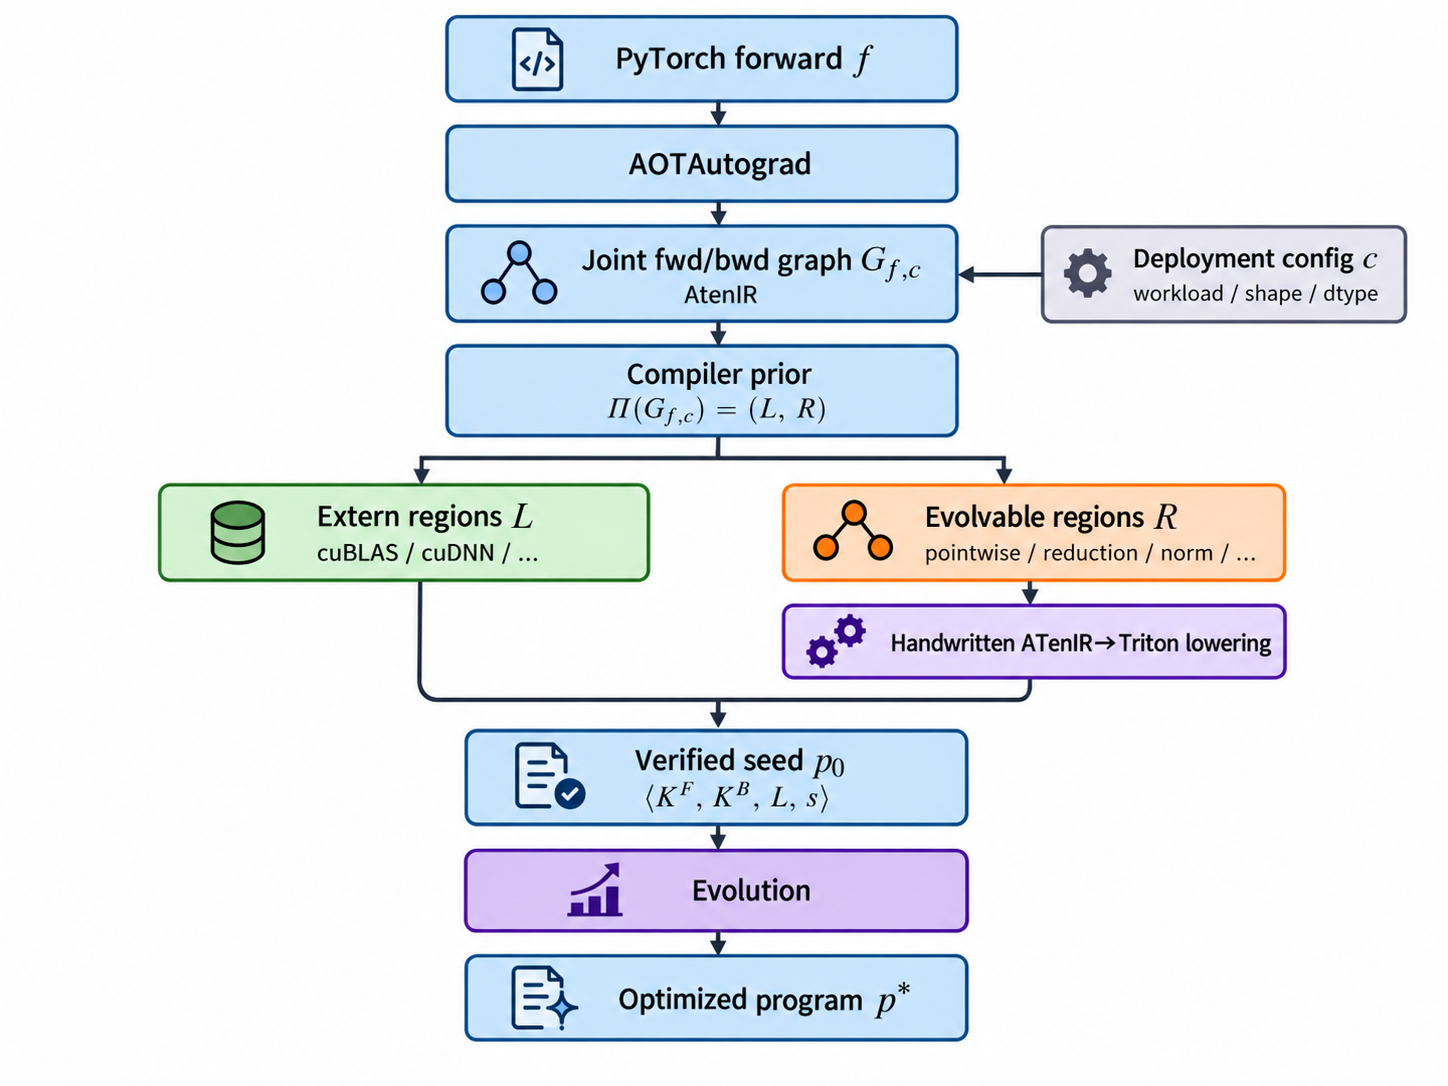
\includegraphics[width=\linewidth]{figures/evograd_pipeline.png}
%     \caption{Overview of \method. AOTAutograd produces a joint forward--backward ATen graph $G_{f,c}$. Compiler-guided partitioning identifies preserved external-library regions $L$ and evolvable semantic regions $R$. Handwritten AtenIR-to-Triton transformations resynthesize $R$, and the resulting kernels are combined with $L$ to form the seed program $p_0$. Evolution jointly optimizes the generated forward and backward implementations and their saved-state policy, with $L$ held fixed.}
%     \label{fig:evograd_pipeline}
% \end{figure}

% \subsection{Compiler-Aware AtenIR Seed Synthesis}
% \label{sec:seed_synthesis}

% \paragraph{Autograd semantic extraction.}
% Given a user-provided PyTorch forward function, \method uses AOTAutograd to derive the corresponding forward and backward computation under deployment configuration $c$. We represent this computation through AtenIR, a graph of ATen operators such as \texttt{aten.add}, \texttt{aten.sum}, and \texttt{aten.mm}. AtenIR captures the required ATen operations and their data dependencies without committing to kernel boundaries or schedules. We initialize the saved-state interface by applying PyTorch's \texttt{min\_cut\_rematerialization\_partition} to the AOTAutograd joint graph, while allowing the saved-state policy to change during subsequent evolution.

% \paragraph{Compiler-aware partitioning.}
% Not every region of the computation should be resynthesized. \method inspects TorchInductor's lowering decisions and partitions the joint graph as
% \begin{equation}
%     \Pi(G_{f,c}) = (L,R),
%     \label{eq:partition}
% \end{equation}
% where $L$ contains regions mapped to external vendor implementations and $R$ contains the remaining computation. In particular, computations such as standard dense GEMMs and convolutions can remain backed by mature libraries such as cuBLAS and cuDNN, avoiding unnecessary search over implementations that are already highly optimized.

% \paragraph{Semantic resynthesis.}
% For the evolvable region $R$, \method returns to its AtenIR representation rather than directly adopting the Triton kernels generated by Inductor. Handwritten lowering rules map supported AtenIR operations to pre-implemented Triton primitives and generate host-side code that invokes them according to the graph's data dependencies. Together, the primitives and their host-side helpers implement the required operator semantics, including broadcasting, dtype conversion, and reduction behavior. This process deterministically constructs a runnable starting point without LLM-based synthesis or cross-operator fusion. These primitive boundaries initialize the seed but remain open to rewriting during evolution. The synthesized forward and backward kernels are then combined with the preserved external-library regions to construct an initial autograd-compatible program
% \begin{equation}
%     p_0 =
%     \left\langle
%         K_0^F,\,
%         K_0^B,\,
%         L,\,
%         s_0
%     \right\rangle,
%     \label{eq:seed_program}
% \end{equation}
% where $K_0^F$ and $K_0^B$ denote the synthesized forward and backward kernels together with their host-side orchestration, $L$ denotes preserved external-library calls, and $s_0$ denotes the state passed from forward to backward. Appendix~\ref{app:seed_example} illustrates the resulting seed
% using a masked linear map, showing the preserved library calls,
% synthesized Triton computation, and forward--backward saved-state interface. 

% \subsection{Evolutionary Optimization}
% \label{sec:evolution}

% Starting from the verified seed $p_0$, \method uses OpenEvolve
% to optimize the objective in Equation~\ref{eq:objective}.
% The search can modify the synthesized Triton kernels,
% their host-side orchestration, and the saved-state policy,
% while preserving the compiler-selected external-library calls
% and public autograd interface. Candidates undergo search-time
% correctness checks before performance measurement; those that
% fail are rejected, while valid candidates receive the fitness
% score defined in Equation~\ref{eq:score} to guide subsequent search.
% Selected final candidates undergo the applicable verification
% and evaluation stages defined by \bench.

% \begin{figure*}[t]
%     \centering
%     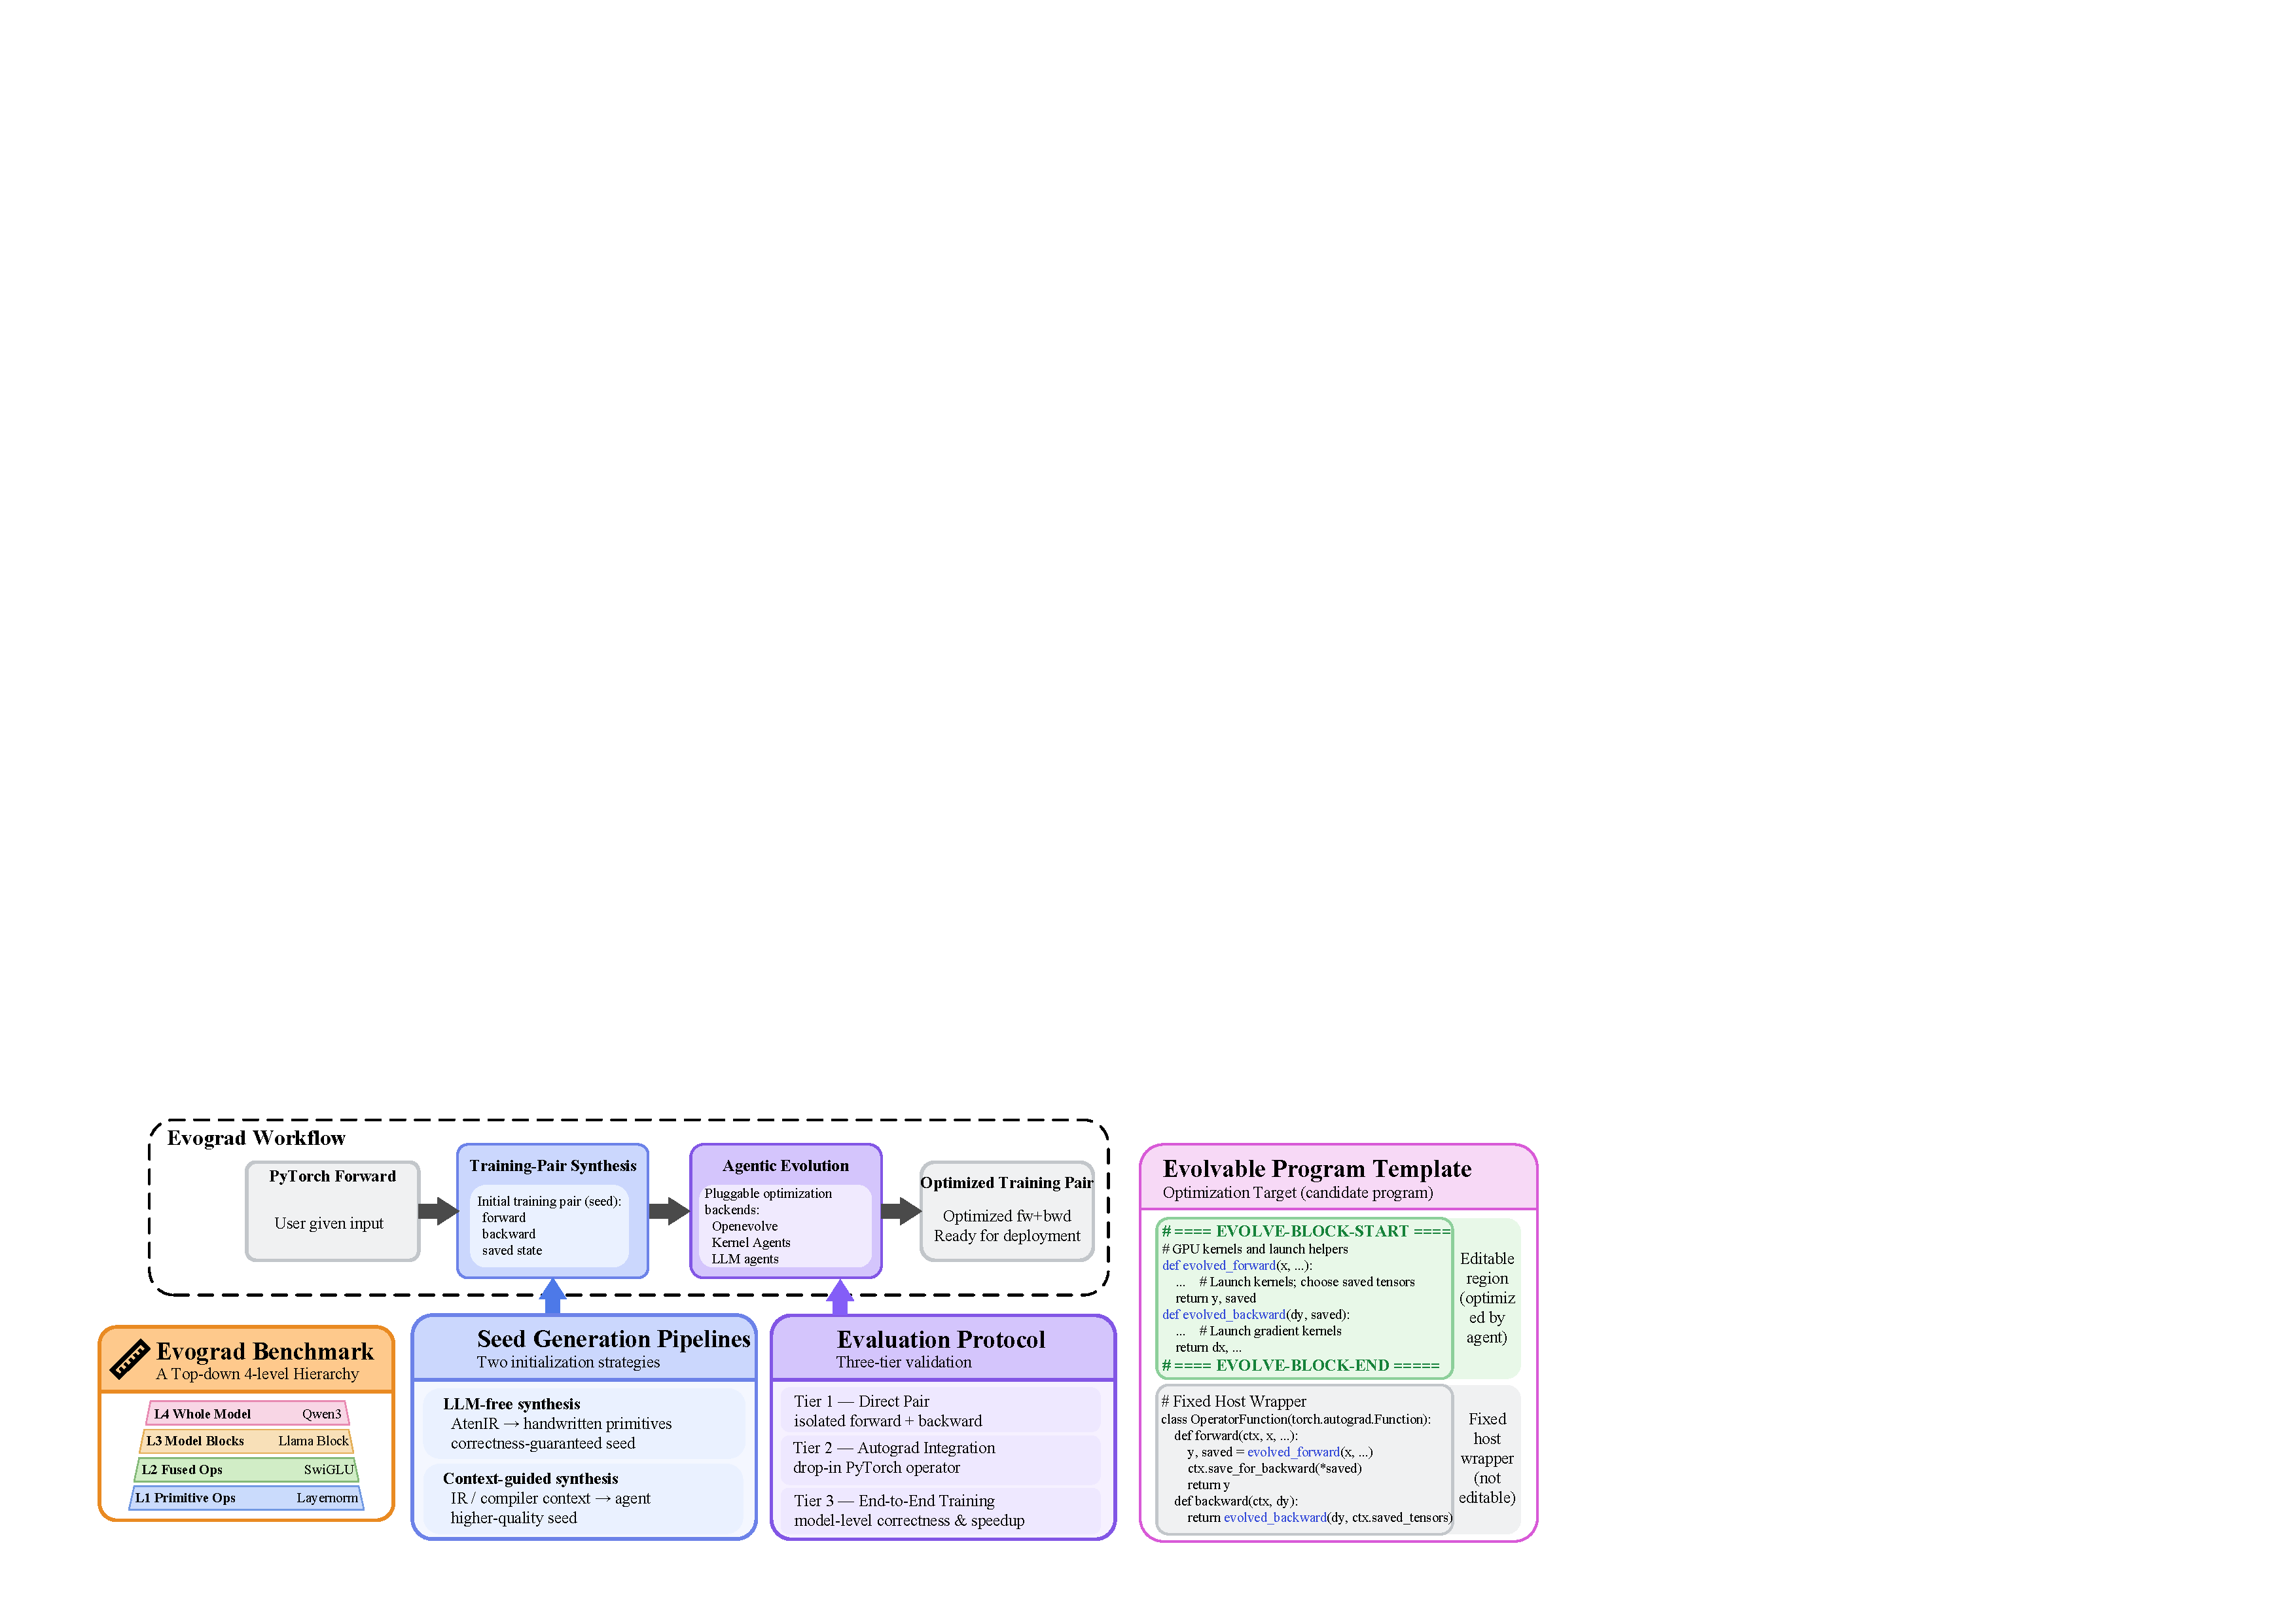
\includegraphics[width=\textwidth]{figures/overview_910.pdf}
%     \caption{Overview of our system. \ahan{Some feedback. (1) Currently each box just states, via words, what is going on. I find this unimformative. We need to diagramatically show, in each box, what is going on. To give a concrete example for agentic evolution we can show some starting code snippet then an ellipses ``..." some intermediate code-snippet showing that it has changed (this is just an example to show how, rather than state what, we are doing). In fact we can show an entry code-snippet in pytorch and show how it is changed in each step, this may be more informative compared to just using words. (2) I am not a big fan of this color scheme, can we use darker colors. (3) You can use the paper X-MoE as a reference: https://arxiv.org/pdf/2508.13337 (See figure 5 for what I mean).} }
%     \label{fig:overview}
% \end{figure*}

% \begin{figure*}[t]
%     \centering
%     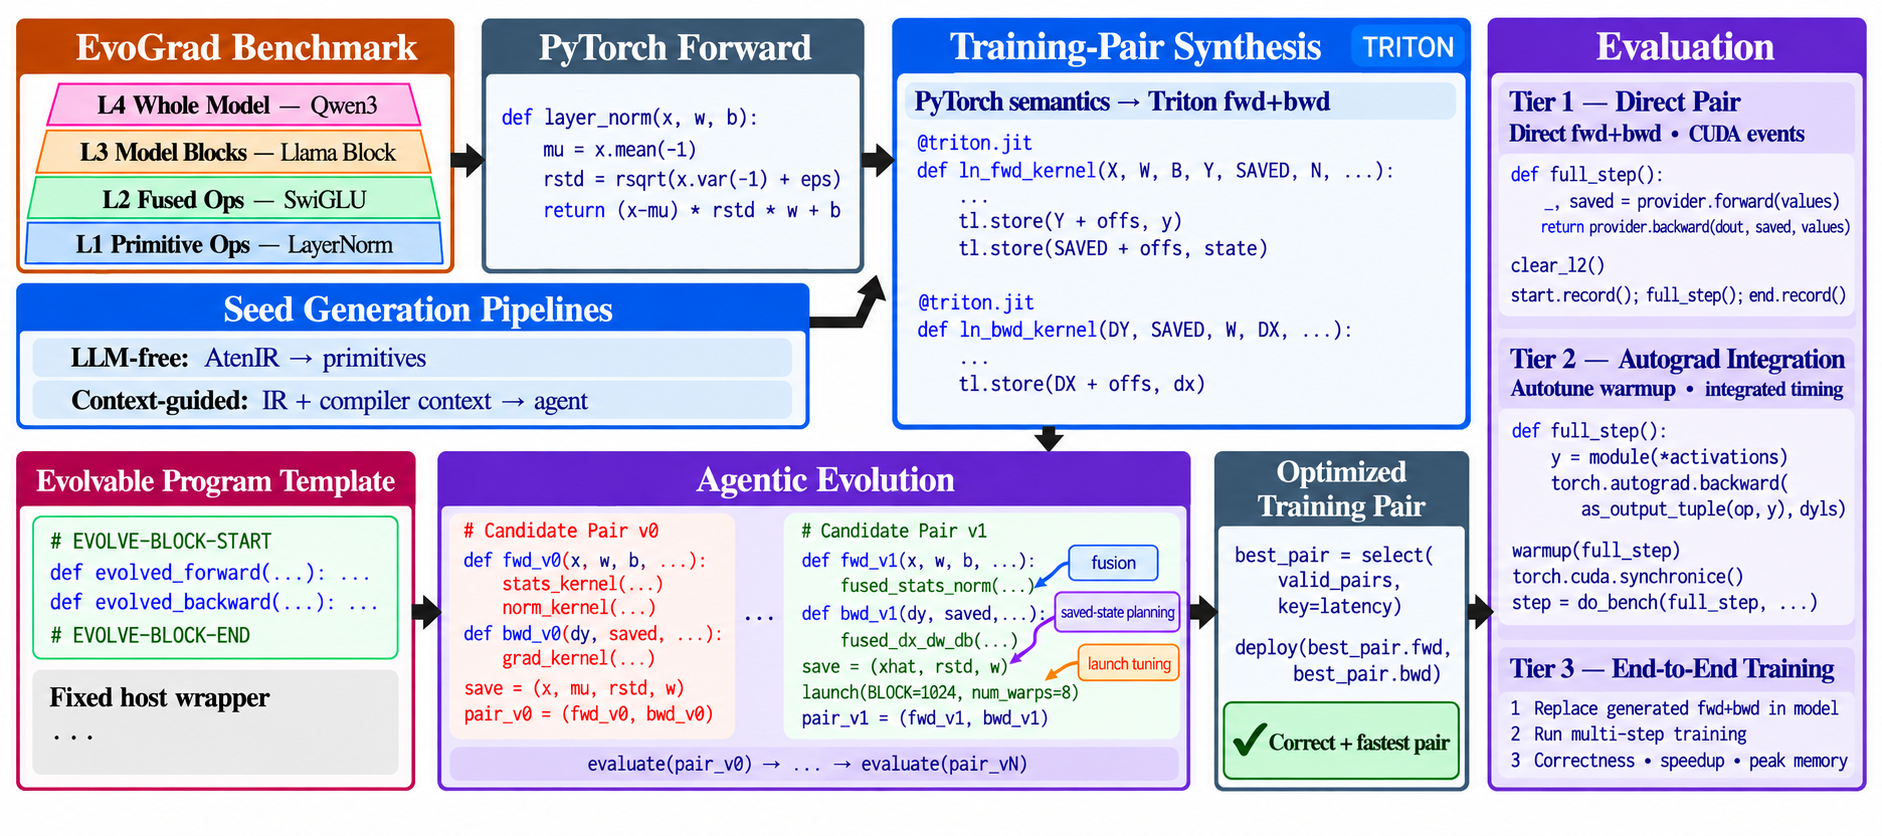
\includegraphics[width=\textwidth]{figures/new_overview.png}
%     \caption{Overview of our system.}
%     \label{fig:overview}
% \end{figure*}

% \ahan{As it's written write now. It's unclear why EvoGrad is needed. The flow introduces ADBench, however, does not state anything as to the problems it exposes. It would be nice to say something like ``hey, now that we've established this benchmark, existing methods sort of suck at AD, spedning many cycles just generating correct programs, resulting in low performance".} \haochen{Word description of the agent benchmarking results. Detailed results are in experiemnt section. }
% Given a task $(f,c)$ specified in Section~\ref{sec:benchmark-task}, \method searches the permitted implementation space $\mathcal{P}_{f,c}$ using a fitness function that combines execution performance and saved-state memory. Candidates remain subject to the forward--backward contract and verification requirements defined by \bench.

% \paragraph{Performance fitness.}
% Let $T_p^{\mathrm{bwd}}(c)$ and $T_p^{\mathrm{full}}(c)$ denote the backward-only and complete forward--backward execution times of candidate $p$, respectively, with $T_{\mathrm{base}}^{\mathrm{bwd}}(c)$ and $T_{\mathrm{base}}^{\mathrm{full}}(c)$ denoting the corresponding performance-baseline times. We define the effective speedup as
% \begin{equation}
%     r(p;c) =
%     \min\!\left(
%         \frac{T_{\mathrm{base}}^{\mathrm{bwd}}(c)}
%              {T_p^{\mathrm{bwd}}(c)},
%         \frac{T_{\mathrm{base}}^{\mathrm{full}}(c)}
%              {T_p^{\mathrm{full}}(c)}
%     \right).
%     \label{eq:effective_speedup}
% \end{equation}
% Using the minimum prevents gains in one execution mode from masking a regression in the other within the performance term.

% \paragraph{Memory penalty.}
% We normalize the logical size of tensors retained for backward by the size of the task's declared memory inputs, defining $R_{\mathrm{saved}}(p;c)=M_p^{\mathrm{saved}}(c)/M_{\mathrm{input}}(c)$. The candidate's fitness is
% \begin{equation}
%     \operatorname{Score}(p;c)
%     =
%     \frac{r(p;c)}
%          {1+\lambda R_{\mathrm{saved}}(p;c)},
%     \label{eq:score}
% \end{equation}
% where $\lambda \geq 0$ controls the penalty for saved memory. This score balances computational speedup against the state retained for backward, allowing recomputation and caching strategies to be compared under the same objective.

% \paragraph{Search objective.}
% The optimization objective is
% \begin{equation}
%     p^\star
%     \in
%     \operatorname*{arg\,max}_{p\in\mathcal{P}_{f,c}}
%     \operatorname{Score}(p;c)
%     \quad \text{subject to} \quad
%     \mathcal{V}(p,f,c)=1,
%     \label{eq:objective}
% \end{equation}
% where $\mathcal{V}$ is the complete verification predicate defined in Eq.~\eqref{eq:validity}. Starting from a seed implementation, \method uses LLM-generated transformations and evaluation feedback to approximate this objective. Search-time checks screen candidates before fitness evaluation; selected candidates must complete the remaining deployment and integration gates before final acceptance. We next describe how \method constructs seeds and organizes candidate transformations.

% \paragraph{Seed structure.}
% Listing~\ref{lst:seed_code_example} illustrates these components using a masked linear map $f(X,W,M)=(XW)\odot M$, where $M$ is a nondifferentiable mask. In the illustrated configuration, the compiler assigns the forward GEMM and the two backward GEMMs to external implementations, forming $L$, while the elementwise multiplications belong to $R$. The same handwritten multiplication primitive is reused by the forward and backward computations. The external-library wrappers and the outer autograd adapter remain fixed, while the primitive kernels, their launch helpers, and the forward--backward orchestration are evolvable. Evolution can therefore replace the initial primitive calls with new implementations and revise the saved-state policy without changing the public autograd interface.


% \ahan{This code listing, though a good start, is too detailed. You don't need to stick to pure Python syntax, you can make it more conscise and readable if you deviate slightly from it.}
% \begin{lstlisting}[
%     language=Python,
%     basicstyle=\ttfamily\scriptsize,
%     columns=fullflexible,
%     keepspaces=true,
%     showstringspaces=false,
%     breaklines=true,
%     frame=single,
%     captionpos=b,
%     caption={Illustrative seed for $f(X,W,M)=(XW)\odot M$. The external-library implementation and autograd adapter are fixed; the Triton primitive, launch helper, and forward--backward orchestration are evolvable. The three preserved GEMM call sites share one displayed wrapper for compactness. Configuration checks and per-region preservation metadata are omitted.},
%     label={lst:seed_code_example}
% ]
% import torch
% import triton
% import triton.language as tl
% from torch._inductor.select_algorithm import extern_kernels

% # Fixed external-library implementation: L.
% def library_mm(a, b):
%     with torch.no_grad():
%         out = torch.empty(
%             (a.shape[0], b.shape[1]),
%             device=a.device, dtype=a.dtype,
%         )
%         extern_kernels.mm(a, b, out=out)
%         return out

% # EVOLVE-BLOCK-START

% # Initial handwritten Triton multiplication primitive.
% @triton.jit
% def _mul_kernel(A, B, OUT, N, BLOCK: tl.constexpr):
%     offsets = tl.program_id(0) * BLOCK + tl.arange(0, BLOCK)
%     mask = offsets < N
%     a = tl.load(A + offsets, mask=mask, other=0.0)
%     b = tl.load(B + offsets, mask=mask, other=0.0)
%     tl.store(OUT + offsets, a * b, mask=mask)

% # Lowering: aten.mul -> host helper -> Triton kernel.
% def mul_tt(a, b):
%     dtype = torch.result_type(a, b)
%     a, b = torch.broadcast_tensors(a, b)
%     a = a.to(dtype).contiguous()
%     b = b.to(dtype).contiguous()
%     out = torch.empty_like(a)
%     grid = (triton.cdiv(out.numel(), 256),)
%     _mul_kernel[grid](a, b, out, out.numel(), BLOCK=256)
%     return out

% # Evolvable forward orchestration and saved state.
% def forward_with_saved(x, w, mask):
%     z = library_mm(x, w)             # Preserved L.
%     y = mul_tt(z, mask)              # Lowered R.
%     return y, (x, w, mask)

% # Evolvable backward orchestration.
% def backward_from_saved(dy, saved):
%     x, w, mask = saved
%     dz = mul_tt(dy, mask)            # Lowered R.
%     dx = library_mm(dz, w.t())       # Preserved L.
%     dw = library_mm(x.t(), dz)       # Preserved L.
%     return dx, dw

% # EVOLVE-BLOCK-END

% # Fixed host adapter for PyTorch autograd.
% class MaskedLinearFunction(torch.autograd.Function):
%     @staticmethod
%     def forward(ctx, x, w, mask):
%         y, saved = forward_with_saved(x, w, mask)
%         ctx.save_for_backward(*saved)
%         return y

%     @staticmethod
%     def backward(ctx, dy):
%         dx, dw = backward_from_saved(dy, ctx.saved_tensors)
%         return dx, dw, None          # No gradient for mask.

% def masked_linear(x, w, mask):
%     return MaskedLinearFunction.apply(x, w, mask)
% \end{lstlisting}

% Before entering evolution, the complete seed $p_0$ is checked against the independent PyTorch-autograd oracle under the same deployment configuration. Only seeds satisfying Equation~\ref{eq:validity} are admitted to the optimization stage.

% \subsection{Profiling-Guided Evolution}
% \label{sec:evolution}

% Starting from the verified seed $p_0$, \method uses OpenEvolve to search for higher-performing programs under the objective in Equation~\ref{eq:objective}. Evolution modifies the synthesized portions of the program while preserving the external-library regions identified during seed synthesis. Each generated candidate must first satisfy the same correctness constraint before its performance is considered.

% The default evolutionary loop uses measured execution performance as its optimization signal. To provide more actionable feedback than a scalar score alone, \method periodically profiles promising candidates with NVIDIA Nsight Compute. A lightweight analysis first identifies major hardware bottlenecks, such as insufficient parallelism, limited memory throughput, or low compute utilization. Selected profiling metrics, together with the current program and deployment context, are then provided to an optimization agent to propose a targeted transformation.

% The proposed program is evaluated using the same correctness and performance gates as ordinary evolutionary candidates. If it improves the objective, it is returned to the OpenEvolve population and becomes available for subsequent search. In this way, profiling feedback supplements broad evolutionary exploration with hardware-specific optimization guidance while leaving correctness and candidate selection under executable evaluation.


% \subsection{Remaining Design Questions}

% \paragraph{Seed-synthesis ablation.} We need an ablation to validate the design choice behind our compiler-aware AtenIR seed synthesis. As discussed, we should compare against two alternative paths: (1) directly evolving compiler-generated Inductor kernels, and (2) synthesizing from AtenIR without compiler-aware partitioning. These comparisons can help isolate the benefit of preserving strong compiler decisions while retaining semantic-level freedom for the remaining computation.

% \paragraph{Evolution agent.} The current draft only describes profiling-guided evolution at a high level. We still need to specify how the evolution agent consumes execution and profiling feedback, identifies optimization opportunities, proposes program transformations, and interacts with the OpenEvolve population. In particular, we should distinguish the hard constraints that every candidate must satisfy from the optimization opportunities that the agent is encouraged to explore.

% \paragraph{Integrating benchmark feedback into optimization.} We also plan to connect the benchmark hierarchy more directly to the optimization framework. For higher-level workloads such as Level-3 cases, instead of synthesizing the entire workload from scratch, we may first optimize lower-level components and compose the higher-level case from these optimized building blocks. Conversely, higher-level evaluation can provide feedback to lower-level optimization. Our current evolution loop is primarily guided by direct forward--backward measurements from Tier-1 evaluation, but the final objective is end-to-end training performance. We should therefore investigate whether Tier-3 signals, such as end-to-end training latency and model-level correctness, can be fed back into evolution for an additional optimization stage targeted directly at deployment-level performance.

% \subsection{Evolution Seed Synthesis}

% \ahan{Another question while reading this. PyTorch-2 inductor automatically code-generates Triton. Why don't we just use those kernels and evolve those rather than do this whole Aten-IR based code-gen? Do we want to motivate why we're doing it this way instead? I see that you compare against naive LLM generated forward baseline, but perhaps we want to talk about this? Just a thought.} \haochen{Added a discussion for this. The pytorch-2 seed generation pipeline is introduced here, while the ablation results are included in 7.}


% \haochen{One thing I'm not sure about the outline of 4.2 and 4.3 is that whether we should include all the methods / agentic frameworks we studied here, or include them in ablations in section 7. I think a reasonable arrangement in my perspective is to include the one final pipeline (after we made the decision) in section 4 along with its advantage, and move the discussions of other possible solutions to section 7. Right now in 4.2 we included all possible ways to do seed synthesis. Please correct me if I misunderstood. }
% \minjia{Yes, we only show the best performing solution in the design. If some components are inspired by other work, we make it explicit. Then we can conduct ablation studies in the evaluation analysis section to show the importance of those components. }

% We explored two different pipelines to generate the initial program for the evolving agent to improve on. In the agent-guided pipeline, a compact summary of the backward AtenIR graph is provided to an LLM that generates a fused Triton seed. This pipeline is flexible, but correctness is not guaranteed and may require multiple generate–evaluate–repair iterations, increasing token and search cost. In the llm-free pipeline, we hand-write and verify Triton kernels for a supported set of ATen operators, then compose these kernels according to the AtenIR data dependencies. This produces a correctness-guaranteed, initially unfused backward seed. Beyond avoiding the repair loop, the structured seed provides evolution with a reliable starting program and reduces the risk of premature convergence to a poor local optimum.

% \subsection{Evolving Agent}
% \subsection{Shape Dispatch}

% \method builds on OpenEvolve as the underlying search engine and augments
% score-based evolution with hardware profiling feedback. Every few iterations, we use the profiling results to optimize the current evolved kernel. A lightweight deterministic roofline analysis first classifies the
% kernel as underutilized, memory-bound, or compute-bound using SM and DRAM
% throughput. Only candidates with meaningful optimization headroom are passed to
% an analysis agent, which combines the roofline result, selected NCU metrics,
% GPU specifications, and benchmark context to produce structured bottleneck
% diagnoses and concrete optimization suggestions. A generation agent then
% revises the program under fixed interface and saved-tensor constraints, so the
% profiling feedback guides performance optimization without changing the task
% contract. The optimized kernel, if scores higher than the origin kernel, would silently replace the original kernel in OpenEvolve's candidate pool to fuel future free exploration. 

% \method treats input shape as a first-class optimization dimension. It
% separately evolves specialists for small and large shapes, evaluates the
% resulting candidates over the full deployment grid, and selects a contiguous
% dispatch threshold from measured performance. The final output is a single
% all-in-one program that dispatches to the appropriate specialist at runtime.
% Our current LayerNorm experiments show that two shape regimes capture most of
% the available gain over a single mixed-shape implementation, while introducing
% a third regime yields only limited additional benefit.





